\documentclass[dvipdfmx]{standalone}
\usepackage{plext}
\usepackage[T1]{fontenc}
\usepackage{newtxtext, newtxmath}

\usepackage{tikz} % xcolor -> graphicx -> tikz

\begin{document}
  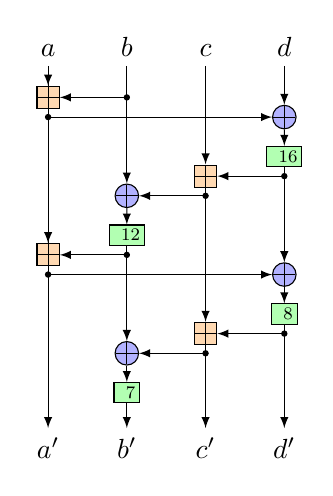
\begin{tikzpicture}[> = latex]

    \tikzset{
      XOR/.style={
        scale=0.9,fill=blue!30,
        draw,circle,append after command={
          [shorten >=\pgflinewidth, shorten <=\pgflinewidth,]
          (\tikzlastnode.north) edge (\tikzlastnode.south)
          (\tikzlastnode.east) edge (\tikzlastnode.west)
        }
      },
      ADD/.style={
        scale=1.2,fill=orange!30,
        draw,rectangle,append after command={
          [shorten >=\pgflinewidth, shorten <=\pgflinewidth,]
          (\tikzlastnode.north) edge (\tikzlastnode.south)
          (\tikzlastnode.east) edge (\tikzlastnode.west)
        }
      },
      ROTATE/.style={
        scale=0.8,fill=green!30,
        draw,rectangle,inner sep=2pt
      },
      DOT/.style={
        scale=0.2,
        draw,circle,fill=black
      }
    }

    % --- nodes ---

    \node at (0,0) [above] (a) {$a$};
    \node at (1,0) [above] (b) {$b$};
    \node at (2,0) [above] (c) {$c$};
    \node at (3,0) [above] (d) {$d$};

    \def\ax{0.25}
    \def\xr{0.5}
    \def\ra{0.25}
    \node at (0,-0.4) (a1) [ADD] {};
    \node at (3,-0.4-\ax) (d1) [XOR] {};
    \node at (3,-0.4-\ax-\xr) (d2) [ROTATE] {$\lll$ \footnotesize 16};
    \node at (2,-0.4-\ax-\xr-\ra) (c1) [ADD] {};
    \node at (1,-1.4-\ax) (b1) [XOR] {};
    \node at (1,-1.4-\ax-\xr) (b2) [ROTATE] {$\lll$ \footnotesize 12};
    \node at (0,-1.4-\ax-\xr-\ra) (a2) [ADD] {};
    \node at (3,-2.4-\ax) (d3) [XOR] {};
    \node at (3,-2.4-\ax-\xr) (d4) [ROTATE] {$\lll$ \footnotesize 8};
    \node at (2,-2.4-\ax-\xr-\ra) (c2) [ADD] {};
    \node at (1,-3.4-\ax) (b3) [XOR] {};
    \node at (1,-3.4-\ax-\xr) (b4) [ROTATE] {$\lll$ \footnotesize 7};

    \node at (0,-4.6) [below] (a') {$a'$};
    \node at (1,-4.6) [below] (b') {$b'$};
    \node at (2,-4.6) [below] (c') {$c'$};
    \node at (3,-4.6) [below] (d') {$d'$};

    % --- paths ---

    \path[->] (a)  edge (a1) (a1) edge (a2) (a2) edge (a');
    \path[->] (b)  edge (b1) (b1) edge (b2) (b2) edge (b3)
              (b3) edge (b4) (b4) edge (b');
    \path[->] (c)  edge (c1) (c1) edge (c2) (c2) edge (c');
    \path[->] (d)  edge (d1) (d1) edge (d2) (d2) edge (d3)
              (d3) edge (d4) (d4) edge (d');

    \draw[<-] (a1) -| node[DOT] {} (b);
    \draw[<-] (d1) -| node[DOT] {} (a);
    \draw[<-] (c1) -| node[DOT] {} (d2);
    \draw[<-] (b1) -| node[DOT] {} (c1);
    \draw[<-] (a2) -| node[DOT] {} (b2);
    \draw[<-] (d3) -| node[DOT] {} (a1);
    \draw[<-] (c2) -| node[DOT] {} (d4);
    \draw[<-] (b3) -| node[DOT] {} (c2);

  \end{tikzpicture}
\end{document}
